
\documentclass[conference]{IEEEtran}
\IEEEoverridecommandlockouts
\renewcommand{\thesection}{\Roman{section}}
\usepackage{booktabs}
\usepackage{fancyhdr}
\usepackage[usenames, dvipsnames]{xcolor}
\usepackage{colortbl}
\usepackage{caption}
\usepackage{graphicx}
\usepackage{array}
\usepackage{adjustbox}
\usepackage{hyperref,graphicx,color,float}
\definecolor{myblue}{RGB}{10, 150, 200}

\usepackage{cite}
\usepackage{multirow}
\usepackage{amsmath,amssymb,amsfonts}
\usepackage{algorithmic}
\usepackage{graphicx}
\usepackage{textcomp}
\usepackage{comment}
\definecolor{highlightColor}{HTML}{E6FFE6}

% --- packages required by this paper's figures and algorithm ---
\usepackage[ruled,vlined]{algorithm2e}
\usepackage{subcaption}
\usepackage{tikz}
\usetikzlibrary{positioning,arrows.meta,shapes.geometric,calc,fit,backgrounds}
\usepackage{pgfplots}
\pgfplotsset{compat=1.17}
\usepgfplotslibrary{groupplots}
\definecolor{beforeblue}{RGB}{31,119,180}
\definecolor{afterorange}{RGB}{255,127,14}

\usepackage{xcolor}
\def\BibTeX{{\rm B\kern-.05em{\sc i\kern-.025em b}\kern-.08em
    T\kern-.1667em\lower.7ex\hbox{E}\kern-.125emX}}
\begin{comment}

\fancypagestyle{firstpage}{
  \fancyhf{} % Clear all header and footer fields
  \fancyhead[L]{\small Conference Name
 \\ Date, Location}
  \fancyfoot[L]{\small XXX-X-XXXX-XXXX-X/XX/\$XX.00 \copyright20XX IEEE} % Left-align the footer
  \renewcommand{\headrulewidth}{0pt} % Remove the header rule
  \renewcommand{\footrulewidth}{0pt} % Remove the footer rule
}
\end{comment}

\pagestyle{plain} % Apply plain style to other pages

\title{Entangled Enhancement in Modular Autonomous\\
Driving Systems: An Empirical Study of Cascade\\
Effects from Single-Component Retraining}

\author{\IEEEauthorblockN{Rashedul Arefin Ifty, Fumio Machida}
\IEEEauthorblockA{University of Tsukuba\\
Tsukuba, Japan\\
ifty.rashedul@sd.cs.tsukuba.ac.jp, machida@cs.tsukuba.ac.jp}}

\begin{document}
\maketitle
% \thispagestyle{firstpage} % Uncomment together with the firstpage block above to show the conference banner/copyright
\bstctlcite{IEEEexample:BSTcontrol}% disable em-dash for repeated author names

\begin{abstract}
Machine learning systems in autonomous driving are maintained incrementally:
one component is retrained as its domain drifts while the rest stays fixed.
This pattern is incompatible with monolithic end-to-end (E2E) models, in which
the smallest retrainable unit is the entire network. We examine the effect of
retraining a single component of a modular perception--prediction--planning
pipeline under domain shift. The pipeline is C1, a YOLOv11n detector, C2,
a constant-velocity predictor, and C3, a rule-based Intelligent Driver Model
planner. We train C1 on Boston nuScenes scenes, fine-tune it on Singapore
scenes, and measure every component in two modes, \emph{isolated} with
ground-truth inputs and \emph{pipeline} with live upstream inputs, before and
after retraining. We observe two effects related to the analytically modeled
notion of \emph{entangled enhancement}: a non-monotone cascade and a decoupling
between a component's aggregate metric and its interface behavior. Retraining
C1 improved C2's pipeline-mode error by 73.98\% (minADE $15.19 \to 3.95$~m),
yet planning error still worsened by 4.45\% (L2@3s $6.30 \to 6.58$~m), while
C1's own detection metric dropped by 45.66\% (mAP@50 $0.119 \to 0.064$). Since
C1's aggregate metric declined, the run does not meet the strict
entangled-enhancement condition but exhibits the related decoupling and
non-monotonicity. All isolated-mode metrics stayed bit-identical, confirming
that every change
traveled through the component interfaces. From five findings we explain why
aggregate component metrics and pipeline behavior diverge, and propose a
cascade-aware retraining assessment protocol that turns our dual-mode
measurement into an admission decision for component updates.
\end{abstract}

\begin{IEEEkeywords}
machine learning systems, autonomous driving, retraining, cascade effects,
software reliability, modular pipelines, regression testing
\end{IEEEkeywords}

% ============================================================================
\section{Introduction}
% ============================================================================
Most recent autonomous driving research follows the end-to-end (E2E) paradigm,
where a single jointly trained network maps raw sensor input directly to a
driving plan. One survey counts more than 270 E2E driving
papers~\cite{chen2024e2esurvey}, built around flagship architectures such as
UniAD~\cite{hu2023uniad} and VAD~\cite{jiang2023vad}, and on benchmark
leaderboards E2E appears to lead.

Deployed systems, however, are maintained under domain drift, one component at
a time: a perception model is retrained for a new city, a predictor is updated
as agent statistics shift, a planner is revised for new regulations.
Maintenance is thus scoped to components, and the E2E paradigm is ill-suited as
an object of maintenance research for three reasons. First, an E2E model admits
a single retraining action, the entire network, with no component states to
threshold and no selective update; recent repair systems reflect this,
fine-tuning the whole planner on synthetic failure data~\cite{ma2025correctad}
or attaching adapters to avoid catastrophic forgetting~\cite{liu2025r2se}.
Second, cost: a single UniAD training run requires about 144
GPU-hours~\cite{sun2024sparsedrive}, so a study of \emph{repeated} retraining,
the essence of maintenance, is far more expensive than in a modular pipeline.
Third, the cascade effects that make maintenance hazardous do not disappear
inside a monolith but become unobservable; the analysis of hidden technical
debt established that ``changing anything changes everything'' and that
correction cascades arise whenever models consume other models'
outputs~\cite{sculley2015hidden}, which an E2E network conceals behind a single
loss.

\looseness=-1
We therefore adopt a modular pipeline as a requirement of the method:
retraining a single component is only well-posed as a research question in an
architecture with separable, independently retrainable components. This work
builds directly on Wang and Machida~\cite{wang2024compsac}, who model a
two-component MLS as a continuous-time Markov chain and name the failure mode
we study, \emph{entangled enhancement}: improving an upstream component on its
own metric can still degrade the system, because downstream components have
learned to operate on the previous upstream output. A follow-on study casts
this as an availability--continuity trade-off~\cite{wang2025issre}. Both are
stochastic models needing empirical calibration, and no one has yet measured
how a single-component retraining event propagates through a real
perception--prediction--planning pipeline. That is the gap this paper fills.

\looseness=-1
This paper supplies that measurement. We build a three-component pipeline on
the nuScenes dataset~\cite{caesar2020nuscenes}: C1, a
YOLOv11n~\cite{jocher2024yolo11} camera detector, C2, a constant-velocity
trajectory predictor, and C3, a rule-based planner from the Intelligent Driver
Model (IDM) family~\cite{treiber2000idm} whose proposal-and-score design
follows PDM-Closed~\cite{dauner2023parting}. We train C1 on Boston scenes,
fine-tune it on Singapore scenes, a well-known domain gap within nuScenes, and
keep C2 and C3 frozen. The focus is on C1, the retrained unit, and C2, its
direct consumer, whose input interface carries the cascade; C3 gives the
system-level reading. The main instrument is dual-mode evaluation: each
downstream component is measured in \emph{isolated} mode with ground-truth
inputs and \emph{pipeline} mode with live upstream outputs. The gap between the
modes isolates the cascade contribution, and its change across a retraining
event measures the cascade the retraining injects.

Our measurements yield five findings, detailed in Section~\ref{sec:results}:
\begin{itemize}
\item[\textbf{F1.}] \textbf{(Architectural.)} The component-level retraining
question is unobservable in an E2E architecture and unaffordable at E2E training
costs; a modular pipeline is the enabling architecture.
\item[\textbf{F2.}] \textbf{(Isolation.)} The isolation property that stochastic
MLS models assume holds exactly: the isolated-mode metrics of the frozen C2 and
C3 stayed bit-identical across the retraining event.
\item[\textbf{F3.}] \textbf{(Cascade existence.)} Retraining C1 alone produced
large, measurable changes downstream, concentrated at the first C1$\to$C2
interface.
\item[\textbf{F4.}] \textbf{(Entangled enhancement.)} The cascade is not
monotone: the same event improved C2's pipeline error by 73.98\% yet worsened
C3's planning error by 4.45\%.
\item[\textbf{F5.}] \textbf{(Metric decoupling.)} C1's aggregate mAP@50
\emph{dropped} by 45.66\% even as its outputs became more useful to C2, so a
component's own metric is not a reliable admission criterion.
\end{itemize}

\textbf{Contributions.} This paper contributes (1)~a dual-mode measurement
method for retraining-induced cascades in modular MLS, with an isolation
check; (2)~a controlled measurement, to our knowledge the first on a real
perception--prediction--planning pipeline, of a single-component retraining
event under a geographic domain shift, revealing a non-monotone cascade and a
decoupling between aggregate and interface metrics, effects adjacent to but
distinct from the strict entangled-enhancement condition; and (3)~a
cascade-aware retraining assessment protocol (Section~\ref{sec:cara}) with a
coupling factor $\rho$ intended to calibrate the base paper's stochastic
maintenance models~\cite{wang2024compsac,wang2025issre}.

The remainder of the paper is organized as follows.
Section~\ref{sec:related} reviews related work.
Section~\ref{sec:method} formalizes the system model and the dual-mode
methodology. Section~\ref{sec:setup} details the experimental setup.
Section~\ref{sec:results} presents results, and
Section~\ref{sec:discussion} discusses the findings and threats to validity.
Section~\ref{sec:cara} presents the proposed assessment protocol, and
Section~\ref{sec:conclusion} concludes.

% ============================================================================
\section{Related Work}
\label{sec:related}
% ============================================================================

\subsection{End-to-End Driving and Its Maintenance Limits}
UniAD put detection, tracking, mapping, motion forecasting, occupancy
prediction, and planning into a single planning-oriented
network~\cite{hu2023uniad}. VAD replaced dense rasterized scene
representations with vectorized ones for efficiency~\cite{jiang2023vad}.
SparseDrive introduced fully sparse scene representations and reported the
resource profile of the flagship systems: $7.2\times$ faster training and
$5\times$ faster inference than UniAD, whose training takes about 144
GPU-hours~\cite{sun2024sparsedrive}. The main survey of the field lists
interpretability, causal confusion, and robustness under distribution shift
as open challenges, and it does not treat component-level maintenance or
retraining policy at all~\cite{chen2024e2esurvey}.

A recent E2E repair literature addresses maintenance directly. CorrectAD
builds a self-correction loop that diagnoses failures, generates targeted
training video with a diffusion model, and fine-tunes the entire E2E planner
on old plus new data, correcting 62.5\% of failure cases on
nuScenes~\cite{ma2025correctad}. R2SE avoids full-model retraining by freezing
the generalist model and training reinforcement-learned low-rank adapter
specialists on failure regions, motivated by the catastrophic forgetting that
naive fine-tuning causes~\cite{liu2025r2se}. Both reintroduce modular structure
to make maintenance tractable, motivating the modular architecture adopted in
this work.

\subsection{Evaluation of Driving Systems}
Our planning metric is open-loop displacement error on nuScenes, and the
limits of this protocol are well documented. Codevilla et al. showed as early
as 2018 that offline prediction error correlates only weakly with actual
closed-loop driving quality~\cite{codevilla2018offline}. Zhai et al. found
that a trivial MLP using only ego state, with no perception at all, matches
perception-based E2E methods on nuScenes open-loop
L2~\cite{zhai2023rethinking}. Dauner et al. showed that open-loop
ego-forecasting and closed-loop driving are misaligned tasks, and that a
largely rule-based planner, PDM-Closed, outperformed learned
planners~\cite{dauner2023parting}. Their later NAVSIM benchmark provides short-horizon non-reactive metrics that
align far better with closed-loop performance~\cite{dauner2024navsim}. These
critiques target open-loop metrics used to \emph{rank} architectures; our use
is differential (the same frozen planner, same scenes, one upstream change), so
much of that weakness cancels, and we report collision rate alongside L2 and
revisit the caveat in Sections~\ref{sec:discussion} and~\ref{sec:threats}.

\subsection{Model Updates, Regression, and Interface Compatibility}
What we measure at system scale has per-sample analogues in the model-update
literature. Yan et al. showed that model updates cause negative flips, samples
the old model handled correctly that the new model gets wrong, at rates of
4--5\% even between equal-accuracy retrains of identical architectures, and
they proposed positive-congruent training with focal distillation to suppress
them~\cite{yan2021pctraining}. The backward-compatible training of Shen et al.
constrains a new upstream representation model so that unchanged downstream
consumers keep working~\cite{shen2020bct}, which is the same situation as
updating C1 beneath a frozen C2 and C3. On the monitoring side, the data
validation system of Breck et al. runs two-sample distribution tests between
pipeline stages in production~\cite{breck2019data}. On a nuScenes
detector--tracker--predictor stack nearly the same shape as ours, Ivanovic et
al. showed that propagating state uncertainty across the
perception--prediction interface, instead of passing point estimates, improves
forecasting by a wide margin~\cite{ivanovic2022propagating}. These works
provide mitigation techniques; this paper contributes the complementary
controlled measurement of the cascade that such techniques are intended to
mitigate.

\subsection{Reliability Modeling of Machine Learning Systems}
The technical-debt analysis of Sculley et al. introduced CACE, unstable data
dependencies, and correction cascades as qualitative failure modes of ML
systems~\cite{sculley2015hidden}. The base paper for this work, Wang and
Machida~\cite{wang2024compsac}, formalized
imperfect retraining of a two-component MLS as a continuous-time Markov chain,
named entangled enhancement, and compared progressive and conservative
maintenance policies; their follow-on work casts the same problem as an
availability--continuity trade-off~\cite{wang2025issre}. Both are analytical
models whose state space grows as $2^N$ for $N$ components, and both are
calibrated on synthetic transition rates. This paper provides an empirical
counterpart: the isolation property we verify (F2) is the property their state
factorization assumes, and the coupling factor we propose
(Section~\ref{sec:cara}) is a measured statistic that can replace those
synthetic rates.

% ============================================================================
\section{System Model and Methodology}
\label{sec:method}
% ============================================================================

\subsection{Formal Pipeline Model}
We model the driving stack as a composition of three functions,
\begin{equation}
S = C_3 \circ C_2 \circ C_1,
\qquad
S(x) = C_3\bigl(C_2(C_1(x))\bigr),
\label{eq:comp}
\end{equation}
where $x$ is a camera keyframe and the three components carry out the
canonical perception--prediction--planning decomposition:
\begin{itemize}
\item \textbf{C1 (Perception):} $z_1 = C_1(x)$ is a set of detected objects,
each with a class, a position, and an extent in the ego frame.
\item \textbf{C2 (Prediction):} $z_2 = C_2(z_1)$ is, for every detected
object, a forecast trajectory over the next several seconds.
\item \textbf{C3 (Planning):} $z_3 = C_3(z_2)$ is the ego vehicle's planned
trajectory, a sequence of positions over a $3$~s horizon.
\end{itemize}
The intermediate signals $z_1$ and $z_2$ are the pipeline interfaces, and each
is a cascade channel: a change in $C_1$'s output distribution shifts $z_1$,
which its direct consumer $C_2$ then propagates into $z_2$ and $C_3$.
Fig.~\ref{fig:pipeline} shows the pipeline annotated with the before/after
numbers measured in this study. Only $C_1$ is retrained (Boston $\to$
Singapore); the isolated (\emph{iso}) metrics of the frozen $C_2$ and $C_3$
stay constant, while their pipeline (\emph{pipe}) metrics move because their
inputs shift.

\begin{figure}[htbp]
\centering
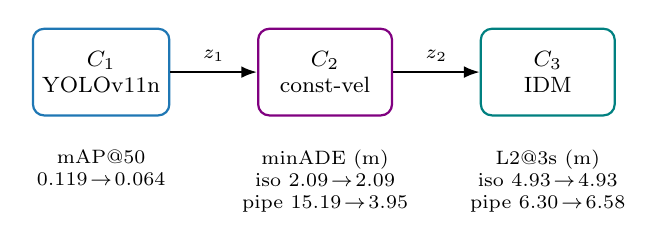
\begin{tikzpicture}[
    font=\footnotesize,
    comp/.style={draw, thick, rounded corners, minimum width=17mm,
                 minimum height=11mm, align=center},
    lbl/.style={align=center, font=\scriptsize},
    arr/.style={-{Latex[length=2mm]}, thick}
]
\node[comp, draw=beforeblue] (c1) {$C_1$\\YOLOv11n};
\node[comp, draw=violet, right=11mm of c1] (c2) {$C_2$\\const-vel};
\node[comp, draw=teal, right=11mm of c2] (c3) {$C_3$\\IDM};
\draw[arr] (c1) -- node[above,font=\scriptsize]{$z_1$} (c2);
\draw[arr] (c2) -- node[above,font=\scriptsize]{$z_2$} (c3);
\node[lbl, below=3mm of c1] {mAP@50\\$0.119\!\to\!0.064$};
\node[lbl, below=3mm of c2] {minADE (m)\\iso $2.09\!\to\!2.09$\\pipe $15.19\!\to\!3.95$};
\node[lbl, below=3mm of c3] {L2@3s (m)\\iso $4.93\!\to\!4.93$\\pipe $6.30\!\to\!6.58$};
\end{tikzpicture}
\caption{Pipeline $C_1\!\to\!C_2\!\to\!C_3$ with before/after numbers.}
\label{fig:pipeline}
\end{figure}

\subsection{Dual-Mode Evaluation}
The core instrument is the measurement of each downstream component in two
modes. Let $z_k^{\star}$ denote the ground-truth value of interface $k$. In
\emph{isolated} mode a component receives ground-truth inputs, so for $C_2$ and
$C_3$ we evaluate
\begin{align}
z_2^{\text{iso}} &= C_2(z_1^{\star}), &
z_3^{\text{iso}} &= C_3(z_2^{\star}).
\label{eq:iso-mode}
\end{align}
In \emph{pipeline} mode a component receives the live output of its upstream
neighbor,
\begin{align}
z_2^{\text{pipe}} &= C_2(C_1(x)), &
z_3^{\text{pipe}} &= C_3(C_2(C_1(x))).
\label{eq:pipe-mode}
\end{align}

For a component $C_k$ with error metric $M_k$ (lower is better), we define the
\emph{cascade gap} at $C_k$ as
\begin{equation}
\Gamma_k = M_k^{\text{pipeline}} - M_k^{\text{isolated}},
\label{eq:gap}
\end{equation}
the part of $C_k$'s error that comes from upstream imperfection rather than
from $C_k$ itself. A retraining event $R$ applied to an upstream component
changes the pipeline metrics. If the system is properly modular, it leaves all
isolated metrics of untouched components unchanged. We call this the
\emph{isolation property}:
\begin{equation}
M_k^{\text{isolated}}(\text{before } R) = M_k^{\text{isolated}}(\text{after } R)
\quad \forall \text{ frozen } C_k.
\label{eq:iso}
\end{equation}
Equation~\eqref{eq:iso} is not assumed but treated as a testable property of
the apparatus: any leakage of the retraining event into a frozen component's
isolated metric indicates contamination, and we verify the equation bit-exactly
in Section~\ref{sec:results}. The cascade \emph{injected} by $R$ at component
$C_k$ is then
\begin{equation}
\Delta_k = M_k^{\text{pipeline}}(\text{after } R) - M_k^{\text{pipeline}}(\text{before } R),
\label{eq:inj}
\end{equation}
which, given~\eqref{eq:iso}, equals the change in the cascade gap $\Gamma_k$.

\subsection{Cascade Diagnostic and Coupling Factor}
\label{sec:diag}
The canonical cascade hypothesis is a conjunction of three conditions: the
retrained upstream component improves on its own metric, the frozen terminal
component is stable in isolation, and it worsens in the pipeline. Writing
$\delta_1$ for the change in the $C_1$ metric (positive denoting improvement)
and using $\Delta_3$ from~\eqref{eq:inj}, we encode the diagnostic as
\begin{equation}
\textsc{cascade} \equiv
\bigl(\delta_1 > 0\bigr)
\ \wedge\
\bigl(\Delta_3^{\text{iso}} = 0\bigr)
\ \wedge\
\bigl(\Delta_3 > \epsilon\bigr),
\label{eq:diag}
\end{equation}
with $\epsilon$ a small noise floor. When~\eqref{eq:diag} holds, the
coupling from the retrained component to the system output is summarized by
the \emph{cascade coupling factor}
\begin{equation}
\rho_{1\to 3} = \frac{\Delta_3}{\delta_1}.
\label{eq:rho-def}
\end{equation}
On a synthetic pipeline with a known planted cascade,
\eqref{eq:diag}--\eqref{eq:rho-def} recover $\rho_{1\to 3} \approx 0.84$, which
serves as an apparatus check prior to the empirical run. As
Section~\ref{sec:results} shows, the empirical outcome does not satisfy the
conjunction~\eqref{eq:diag} in its canonical form: $\delta_1 < 0$ (aggregate
mAP fell) while $\Delta_3 > 0$, so $\rho_{1\to 3}$ is of ambiguous sign. This
mismatch is not a null result but the entangled-enhancement regime itself, and
it is precisely why $\rho$ must be interpreted together with the full cascade
vector rather than as an isolated scalar (Section~\ref{sec:cara}).

\subsection{Single-Component Retraining Under Domain Shift}
\label{sec:experiment}
The experiment retrains only C1:
\begin{enumerate}
\item Train C1 on the source domain (Boston scenes). Freeze C2 and C3
permanently.
\item Measure the five-quantity profile on the target-domain validation set
(Singapore): C1 detection quality (mAP@50), C2-isolated minADE, C2-pipeline
minADE, C3-isolated L2@$\{1,2,3\}$s, C3-pipeline L2@$\{1,2,3\}$s.
\item Fine-tune C1 on the target domain (Singapore scenes), producing the
retrained C1$'$.
\item Re-measure the identical five-quantity profile with C1$'$ in place.
\item Verify the isolation property~\eqref{eq:iso} and compute the injected
cascades~\eqref{eq:inj} at C2 and C3.
\end{enumerate}
The Boston-to-Singapore shift within nuScenes is a genuine and well-studied
domain gap: left- versus right-hand traffic, different vehicle and agent
mixes, and different lighting conditions~\cite{caesar2020nuscenes}.

\subsection{Metrics}
C1 is scored with standard detection metrics (mAP@50, mAP@50-95, precision,
recall) on the target-domain validation images. For $C_2$, the metric is the
minimum average displacement error (minADE). For an agent with forecast
positions $\hat{p}^{(m)}_{t}$ under mode $m$ and ground-truth positions
$p^{\star}_{t}$ over $T$ future steps,
\begin{equation}
\mathrm{minADE} = \min_{m}\ \frac{1}{T}\sum_{t=1}^{T}
\bigl\lVert \hat{p}^{(m)}_{t} - p^{\star}_{t} \bigr\rVert_2 ,
\label{eq:minade}
\end{equation}
averaged over agents. Our deterministic predictor has a single mode, so the
$\min$ collapses to that mode. For $C_3$, the metric is the L2 displacement
error between the planned ego trajectory $\hat{e}_t$ and the human driver's
recorded trajectory $e^{\star}_t$ at horizon $\tau$,
\begin{equation}
\mathrm{L2}@\tau = \bigl\lVert \hat{e}_{\tau} - e^{\star}_{\tau} \bigr\rVert_2 ,
\qquad \tau \in \{1,2,3\}\ \text{s},
\label{eq:l2}
\end{equation}
reported together with collision rate. The C3 metric is the standard nuScenes
open-loop planning protocol used by the E2E
literature~\cite{hu2023uniad,jiang2023vad,zhai2023rethinking}, with the
differential-use caveat discussed in Sections~\ref{sec:related} and
\ref{sec:threats}.

% ============================================================================
\section{Experimental Setup}
\label{sec:setup}
% ============================================================================

\subsection{Dataset and Components}
We use nuScenes-mini v1.0~\cite{caesar2020nuscenes}. Partitioning by recorded
location and splitting each domain into train and validation gives
\texttt{boston\_train}/\texttt{boston\_val} (2/2 scenes) and
\texttt{singapore\_train}/\texttt{singapore\_val} (3/3 scenes); all cascade
measurements use \texttt{singapore\_val} ($n=3$). For C1 training, the 3D box
annotations are projected onto the front-camera keyframes to produce 2D labels
over eight driving classes.

C1 is YOLOv11n~\cite{jocher2024yolo11}, fine-tuned for 10 epochs on
\texttt{boston\_train} from COCO weights, then a further 10 epochs on
\texttt{singapore\_train} starting from the Boston checkpoint; the two
checkpoints are the before/after detectors. At inference, each 2D detection is
lifted to an ego-frame ground position by intersecting its bottom-center pixel
ray with the ground plane, supplying the agent positions $z_1$ that C2
consumes. C2 is a deterministic, parameter-free constant-velocity predictor:
in isolated mode it rolls agents out at their ground-truth velocity, and in
pipeline mode it anchors a zero-velocity rollout at C1's single-frame
detections, so that any change in its pipeline output is attributable solely to
a change in C1.
C3 is a rule-based Intelligent Driver Model~\cite{treiber2000idm}
proposal-and-score planner that selects, from a speed-aware grid of candidate
trajectories $\mathcal{P}$, the one minimizing progress cost plus a soft
proximity penalty against the predicted agent futures $z_2$,
\begin{equation}
\pi^{\star} = \arg\min_{\pi \in \mathcal{P}}\
J_{\text{prog}}(\pi)
\ +\ \lambda \!\!\sum_{a \in z_2} \phi\bigl(d(\pi, a)\bigr),
\label{eq:idm}
\end{equation}
where $d(\pi,a)$ is the closest approach between candidate $\pi$ and agent $a$,
$\phi$ is a soft penalty on proximity, and $\lambda$ weights safety against
progress. This reproduces the PDM-Closed~\cite{dauner2023parting} architecture
without its learned scorer; the dependence of~\eqref{eq:idm} on $z_2$ is the
channel through which perturbed detections reach the plan.

\subsection{Measurement Protocol}
The harness computes the five-quantity profile of Section~\ref{sec:experiment}
for both C1 checkpoints on \texttt{singapore\_val}, with all randomness fixed
across the two runs. Because C2 and C3 have no trainable parameters, the
isolation property~\eqref{eq:iso} can be checked for exact equality rather than
statistical closeness.

% ============================================================================
\section{Results}
\label{sec:results}
% ============================================================================

\subsection{Headline Measurements}
Table~\ref{tab:results} reports the complete before/after profile on
\texttt{singapore\_val}, where ``before'' is the Boston-trained $C_1$ and
``after'' is the Singapore-fine-tuned $C_1$, and Fig.~\ref{fig:tablefull}
plots it. The detection quality of $C_1$ (mAP@50) drops after fine-tuning,
C2-pipeline minADE improves sharply ($15.19 \to 3.95$~m), and C3-pipeline
L2@3s worsens ($6.30 \to 6.58$~m). Both isolated metrics are unchanged, which
is the visual signature of the isolation property~\eqref{eq:iso}.

\begin{table}[htbp]
\caption{Measurements on Singapore validation ($n=3$ scenes).}
\label{tab:results}
\centering
\renewcommand{\arraystretch}{1.2}
\setlength{\tabcolsep}{4pt}
\begin{tabular}{@{}lrrrr@{}}
\toprule
\textbf{Metric} & \textbf{Before} & \textbf{After} & \textbf{$\Delta$} & \textbf{$\Delta$\%} \\
\midrule
C1 mAP@50                & 0.1185  & 0.0644 & $-0.0541$  & $-45.66$ \\
C1 mAP@50-95             & 0.0571  & 0.0258 & $-0.0313$  & $-54.81$ \\
C1 precision             & 0.6845  & 0.6709 & $-0.0136$  & $-1.99$  \\
C1 recall                & 0.0866  & 0.0477 & $-0.0389$  & $-44.92$ \\
C2 iso.\ minADE (m)      & 2.0899  & 2.0899 & $0.0000$   & $0.00$   \\
\textbf{C2 pipe.\ minADE (m)} & \textbf{15.1930} & \textbf{3.9535} & $\mathbf{-11.2395}$ & $\mathbf{-73.98}$ \\
C3 iso.\ L2@1s (m)       & 0.6900  & 0.6900 & $0.0000$   & $0.00$   \\
C3 iso.\ L2@2s (m)       & 2.4944  & 2.4944 & $0.0000$   & $0.00$   \\
C3 iso.\ L2@3s (m)       & 4.9289  & 4.9289 & $0.0000$   & $0.00$   \\
C3 pipe.\ L2@1s (m)      & 1.0396  & 1.0838 & $+0.0442$  & $+4.25$  \\
C3 pipe.\ L2@2s (m)      & 3.5017  & 3.6070 & $+0.1053$  & $+3.01$  \\
\textbf{C3 pipe.\ L2@3s (m)} & \textbf{6.2969} & \textbf{6.5770} & $\mathbf{+0.2801}$ & $\mathbf{+4.45}$ \\
C3 pipe.\ collision rate & 0.000   & 0.000  & $0.0000$   & --- \\
\bottomrule
\end{tabular}
\end{table}

\begin{figure}[htbp]
\centering
% Shared legend row above both panels (manual, always renders, clears titles).
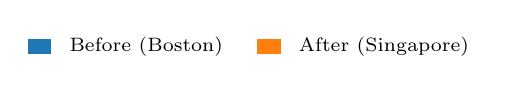
\begin{tikzpicture}
\node[fill=beforeblue, minimum width=3mm, minimum height=2mm, inner sep=0pt] (lb) {};
\node[right=1mm of lb, font=\scriptsize] (lbt) {Before (Boston)};
\node[right=3mm of lbt, fill=afterorange, minimum width=3mm, minimum height=2mm, inner sep=0pt] (la) {};
\node[right=1mm of la, font=\scriptsize] {After (Singapore)};
\end{tikzpicture}\\[0.3ex]
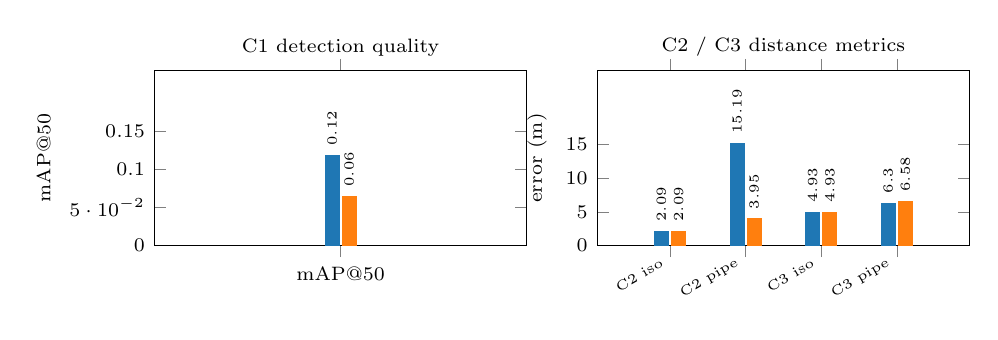
\begin{tikzpicture}
\begin{groupplot}[
  group style={group size=2 by 1, horizontal sep=9mm},
  width=0.52\columnwidth, height=3.8cm,
  ybar=1.2pt, /pgf/bar width=5pt,
  ymin=0, enlarge x limits=0.32,
  tick label style={font=\scriptsize},
  label style={font=\scriptsize},
  title style={font=\scriptsize, yshift=-1ex},
  % Data value labels are rotated vertical (reading bottom-to-top) and sit
  % above each bar, so close/equal pairs never collide.
  nodes near coords, nodes near coords style={font=\tiny, rotate=90,
        anchor=west, /pgf/number format/fixed, /pgf/number format/precision=2},
]
% Panel 1: C1 detection quality
\nextgroupplot[title={C1 detection quality},
  ylabel={mAP@50}, symbolic x coords={mAP@50}, xtick=data, ymax=0.23,
  ytick={0,0.05,0.1,0.15}]
\addplot[fill=beforeblue, draw=beforeblue] coordinates {(mAP@50,0.1185)};
\addplot[fill=afterorange, draw=afterorange] coordinates {(mAP@50,0.0644)};
% Panel 2: C2 / C3 distance metrics. Vertical value labels avoid the
% collisions that the horizontal labels had on equal/close bar pairs.
\nextgroupplot[title={C2 / C3 distance metrics},
  ylabel={error (m)}, ymax=26, ytick={0,5,10,15},
  symbolic x coords={C2 iso,C2 pipe,C3 iso,C3 pipe},
  xtick=data, x tick label style={rotate=30, anchor=east, font=\tiny}]
\addplot[fill=beforeblue, draw=beforeblue]
  coordinates {(C2 iso,2.09) (C2 pipe,15.19) (C3 iso,4.93) (C3 pipe,6.30)};
\addplot[fill=afterorange, draw=afterorange]
  coordinates {(C2 iso,2.09) (C2 pipe,3.95) (C3 iso,4.93) (C3 pipe,6.58)};
\end{groupplot}
\end{tikzpicture}
\caption{Full profile on \texttt{singapore\_val}, before versus after:
(a) C1 detection quality, (b) C2/C3 distance metrics.}
\label{fig:tablefull}
\end{figure}

\subsection{Verification of the Isolation Property (Finding F2)}
The three isolated-mode rows are exactly zero-delta. C2-isolated minADE is
$2.0899$~m in both runs, and C3-isolated L2 is $0.6900 / 2.4944 / 4.9289$~m at
the three horizons in both runs, to every recorded digit. For deterministic,
parameter-free C2 and C3 fed identical ground-truth inputs, this invariance is
expected by construction; we report it as a validity check on the apparatus
rather than as a discovery, since any nonzero delta would have signalled state
or data leakage between the runs. Its role is to certify that the pipeline-mode
deltas in Table~\ref{tab:results} arise solely from the C1 retraining event,
transmitted through the component interfaces, the premise on which the
injected-cascade readings depend.

\subsection{Cascade Concentration at the C1$\to$C2 Interface (Finding F3)}
\looseness=-1
The largest single effect in Table~\ref{tab:results} occurs at the C1$\to$C2
interface. With the Boston-trained C1, C2's pipeline-mode minADE was
$15.1930$~m against an isolated-mode floor of $2.0899$~m, a cascade gap
$\Gamma_2$ of $13.10$~m. This $\Gamma_2$ conflates two sources: C1 detection
error and the loss of velocity information, since C2-isolated uses ground-truth
velocity whereas C2-pipeline uses a zero-velocity rollout
(Section~\ref{sec:setup}); it therefore bounds the combined effect, not
perception error alone. After the Singapore fine-tune, C2-pipeline minADE fell
to $3.9535$~m ($\Gamma_2 = 1.86$~m), a 73.98\% improvement without modifying
C2. The change $\Delta_2 = -11.24$~m is attributable to C1 alone, since the
velocity-information gap is constant across the two runs, so the first
downstream interface dominates the retraining-induced cascade.

\subsection{Simultaneous Degradation at the System Output (Finding F4)}
Even though C2-pipeline improved by 73.98\%, C3-pipeline worsened at every
horizon: $+4.25\%$ at 1~s, $+3.01\%$ at 2~s, and $+4.45\%$ at 3~s ($6.2969$~m
$\to 6.5770$~m, $\Delta_3 = +0.2801$~m). The cascade gap at the planner grew
from $\Gamma_3 = 1.37$~m to $1.65$~m, with collision rate zero in both runs.
The two pipeline-mode deltas therefore carry opposite signs: the retraining
event that improved the planner's inputs degraded its output. Read against the
diagnostic~\eqref{eq:diag}, the run satisfies the isolation clause
($\Delta_3^{\text{iso}}=0$) and the degradation clause
($\Delta_3 = +0.28$~m $> \epsilon$) but \emph{not} the upstream-improvement
clause, because aggregate mAP fell (F5). The run is therefore not a clean
instance of entangled enhancement in the strict sense of the base
paper~\cite{wang2024compsac}, which requires $\delta_1 > 0$; it is the related
non-monotone regime, in which C2's interface improves while the system output
degrades. It is nonetheless a controlled, quantified instance of the
correction-cascade and improvement-deadlock pattern that the technical-debt
literature describes only qualitatively~\cite{sculley2015hidden}.
Fig.~\ref{fig:cascade} illustrates the effect: C3-isolated remains fixed at
$4.93$~m, since the planner
receives identical ground-truth inputs in both runs, while C3-pipeline drifts
from $6.30$ to $6.58$~m.

\begin{figure}[htbp]
\centering
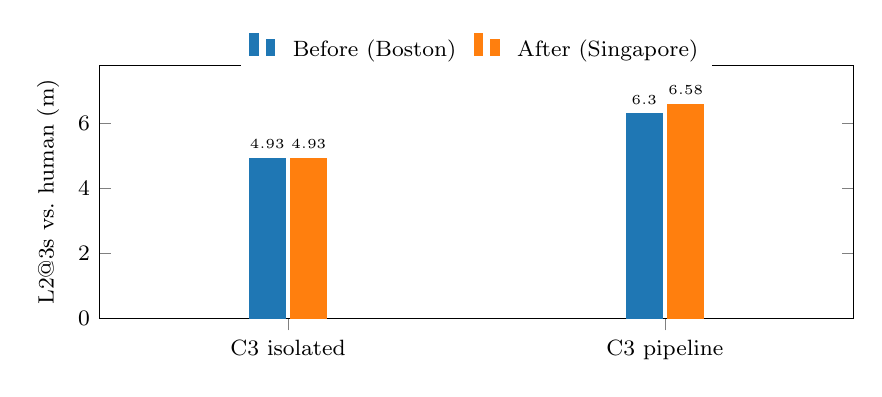
\begin{tikzpicture}
\begin{axis}[
  width=0.92\columnwidth, height=4.8cm,
  ybar=2pt, /pgf/bar width=13pt, ymin=0, ymax=7.8,
  ylabel={L2@3s vs.\ human (m)},
  symbolic x coords={C3 isolated, C3 pipeline}, xtick=data,
  tick label style={font=\footnotesize}, label style={font=\footnotesize},
  enlarge x limits=0.5,
  legend style={at={(0.5,1.15)}, anchor=north, legend columns=2,
                draw=none, font=\footnotesize, column sep=1ex},
  nodes near coords, nodes near coords style={font=\tiny,
        /pgf/number format/fixed, /pgf/number format/precision=2},
]
\addplot[fill=beforeblue, draw=beforeblue]
  coordinates {(C3 isolated,4.93) (C3 pipeline,6.30)};
\addplot[fill=afterorange, draw=afterorange]
  coordinates {(C3 isolated,4.93) (C3 pipeline,6.58)};
\legend{Before (Boston), After (Singapore)}
\end{axis}
\end{tikzpicture}
\caption{Cascade signature on planning: isolated fixed, pipeline drifts.}
\label{fig:cascade}
\end{figure}

\subsection{Aggregate Metric Decoupling at C1 (Finding F5)}
\looseness=-1
Table~\ref{tab:results} exhibits a second inversion. The Singapore-fine-tuned
C1, the checkpoint that improved C2 by 74\%, scores \emph{lower} on its own
aggregate validation metric than its Boston-trained predecessor (mAP@50
$0.1185 \to 0.0644$, $-45.66\%$; recall $0.0866 \to 0.0477$). The immediate
cause is small-data overfitting: the Singapore fine-tune set contains only 119
images (944 instances) with a sparse class mix, and the fine-tuned detector
converges to detection regimes that diverge from the validation label
distribution, as evident in the confusion matrix of Fig.~\ref{fig:confusion},
where most non-car classes collapse into the background row. The cascade,
however, does not propagate through the aggregate score but through the
detection outputs themselves: a detector can lose mAP while emitting outputs
that are more useful to its downstream consumer on the relevant scenes.
Aggregate component metrics and interface behavior therefore decouple, here
moving in opposite directions with large magnitudes on both sides, so a
component's own metric is not a reliable admission criterion. This is the
per-component, system-scale analogue of the negative-flip phenomenon reported
for classifier updates~\cite{yan2021pctraining}.

\begin{figure}[htbp]
\centering
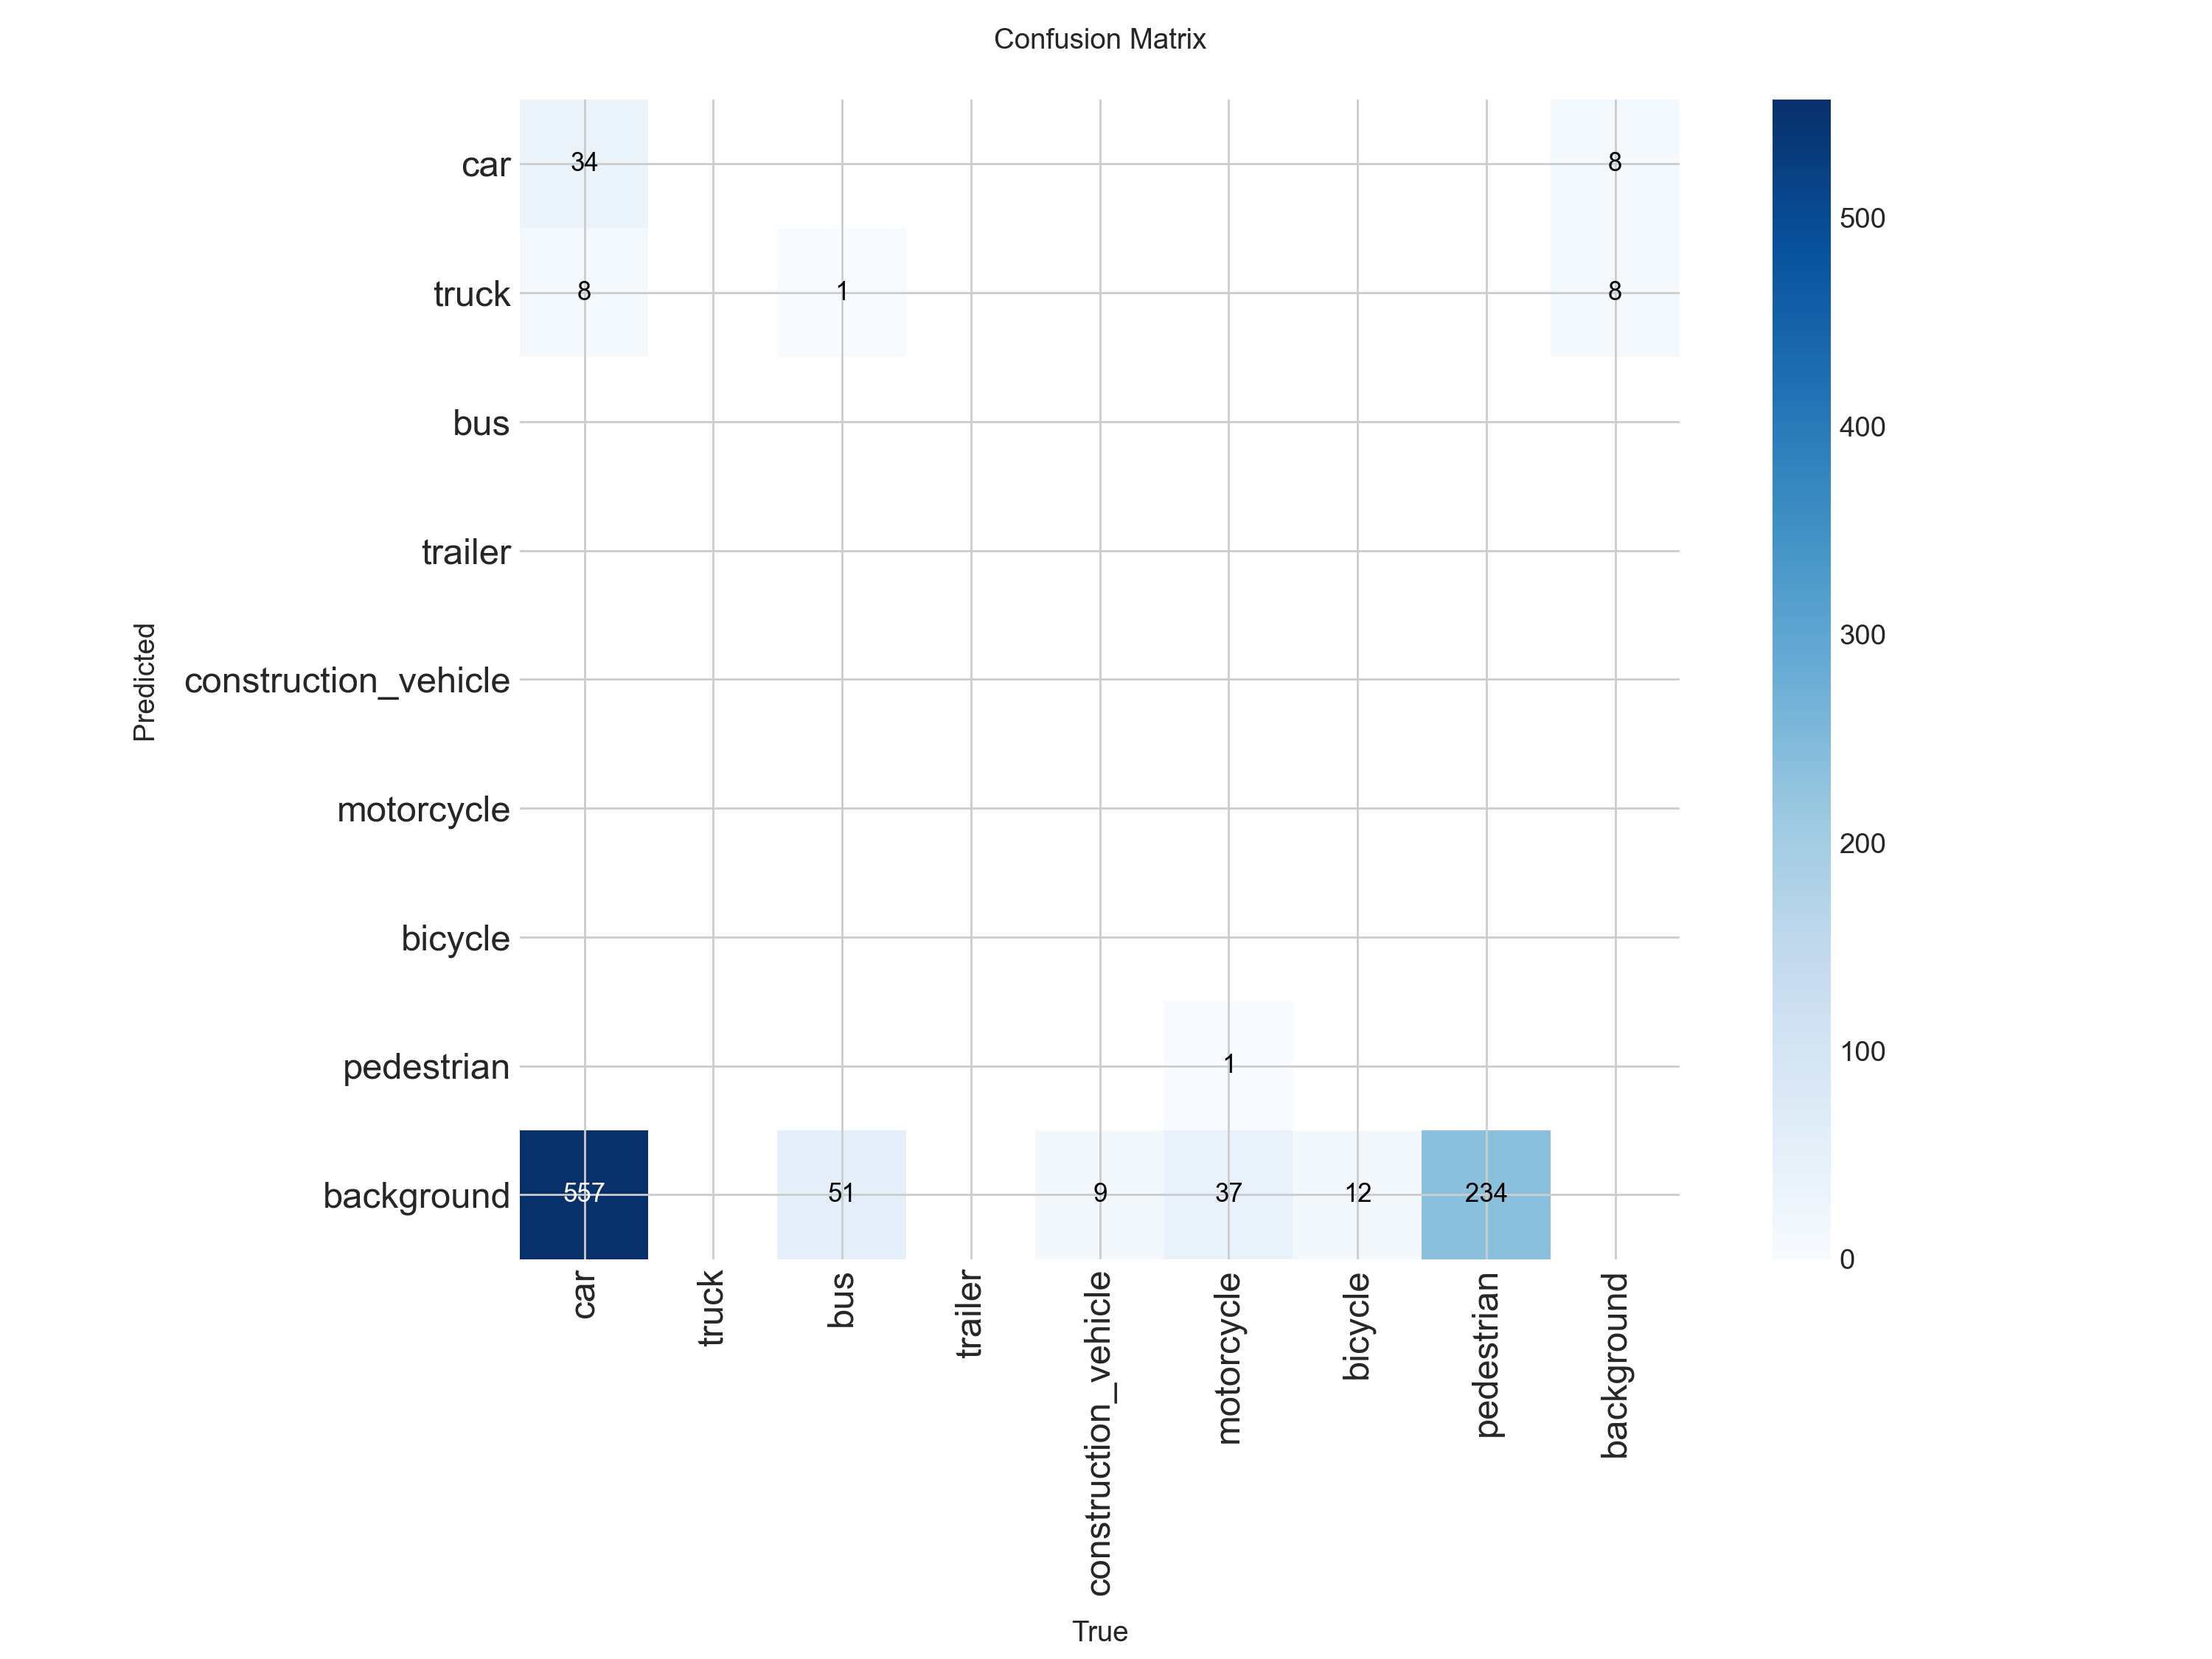
\includegraphics[width=0.92\columnwidth]{figures/fig05_singapore_confusion.png}
\caption{Confusion matrix of the Singapore-fine-tuned $C_1$.}
\label{fig:confusion}
\end{figure}

\subsection{Training Diagnostics}
Both fine-tunes converged within their 10-epoch budgets with monotone loss
decay, as Fig.~\ref{fig:curves} shows for the Boston run: the box,
classification, and distribution-focal losses decrease on both the train and
validation splits, while precision, recall, and mAP@50 increase, with mAP@50
rising from $0.039$ at epoch 1 to $0.119$ at epoch 10. Each fine-tune completes
in under a GPU-minute, several orders of magnitude below the cost of a single
E2E training run~\cite{sun2024sparsedrive}, which is what renders a study of
repeated retraining feasible. Fig.~\ref{fig:qual} shows a qualitative $C_1$
output batch; the cascade propagates through the ego-frame positions of the
detected boxes, which alter the forecasts and hence the plan, independently of
whether the detections differ visibly.

\begin{figure}[htbp]
\centering
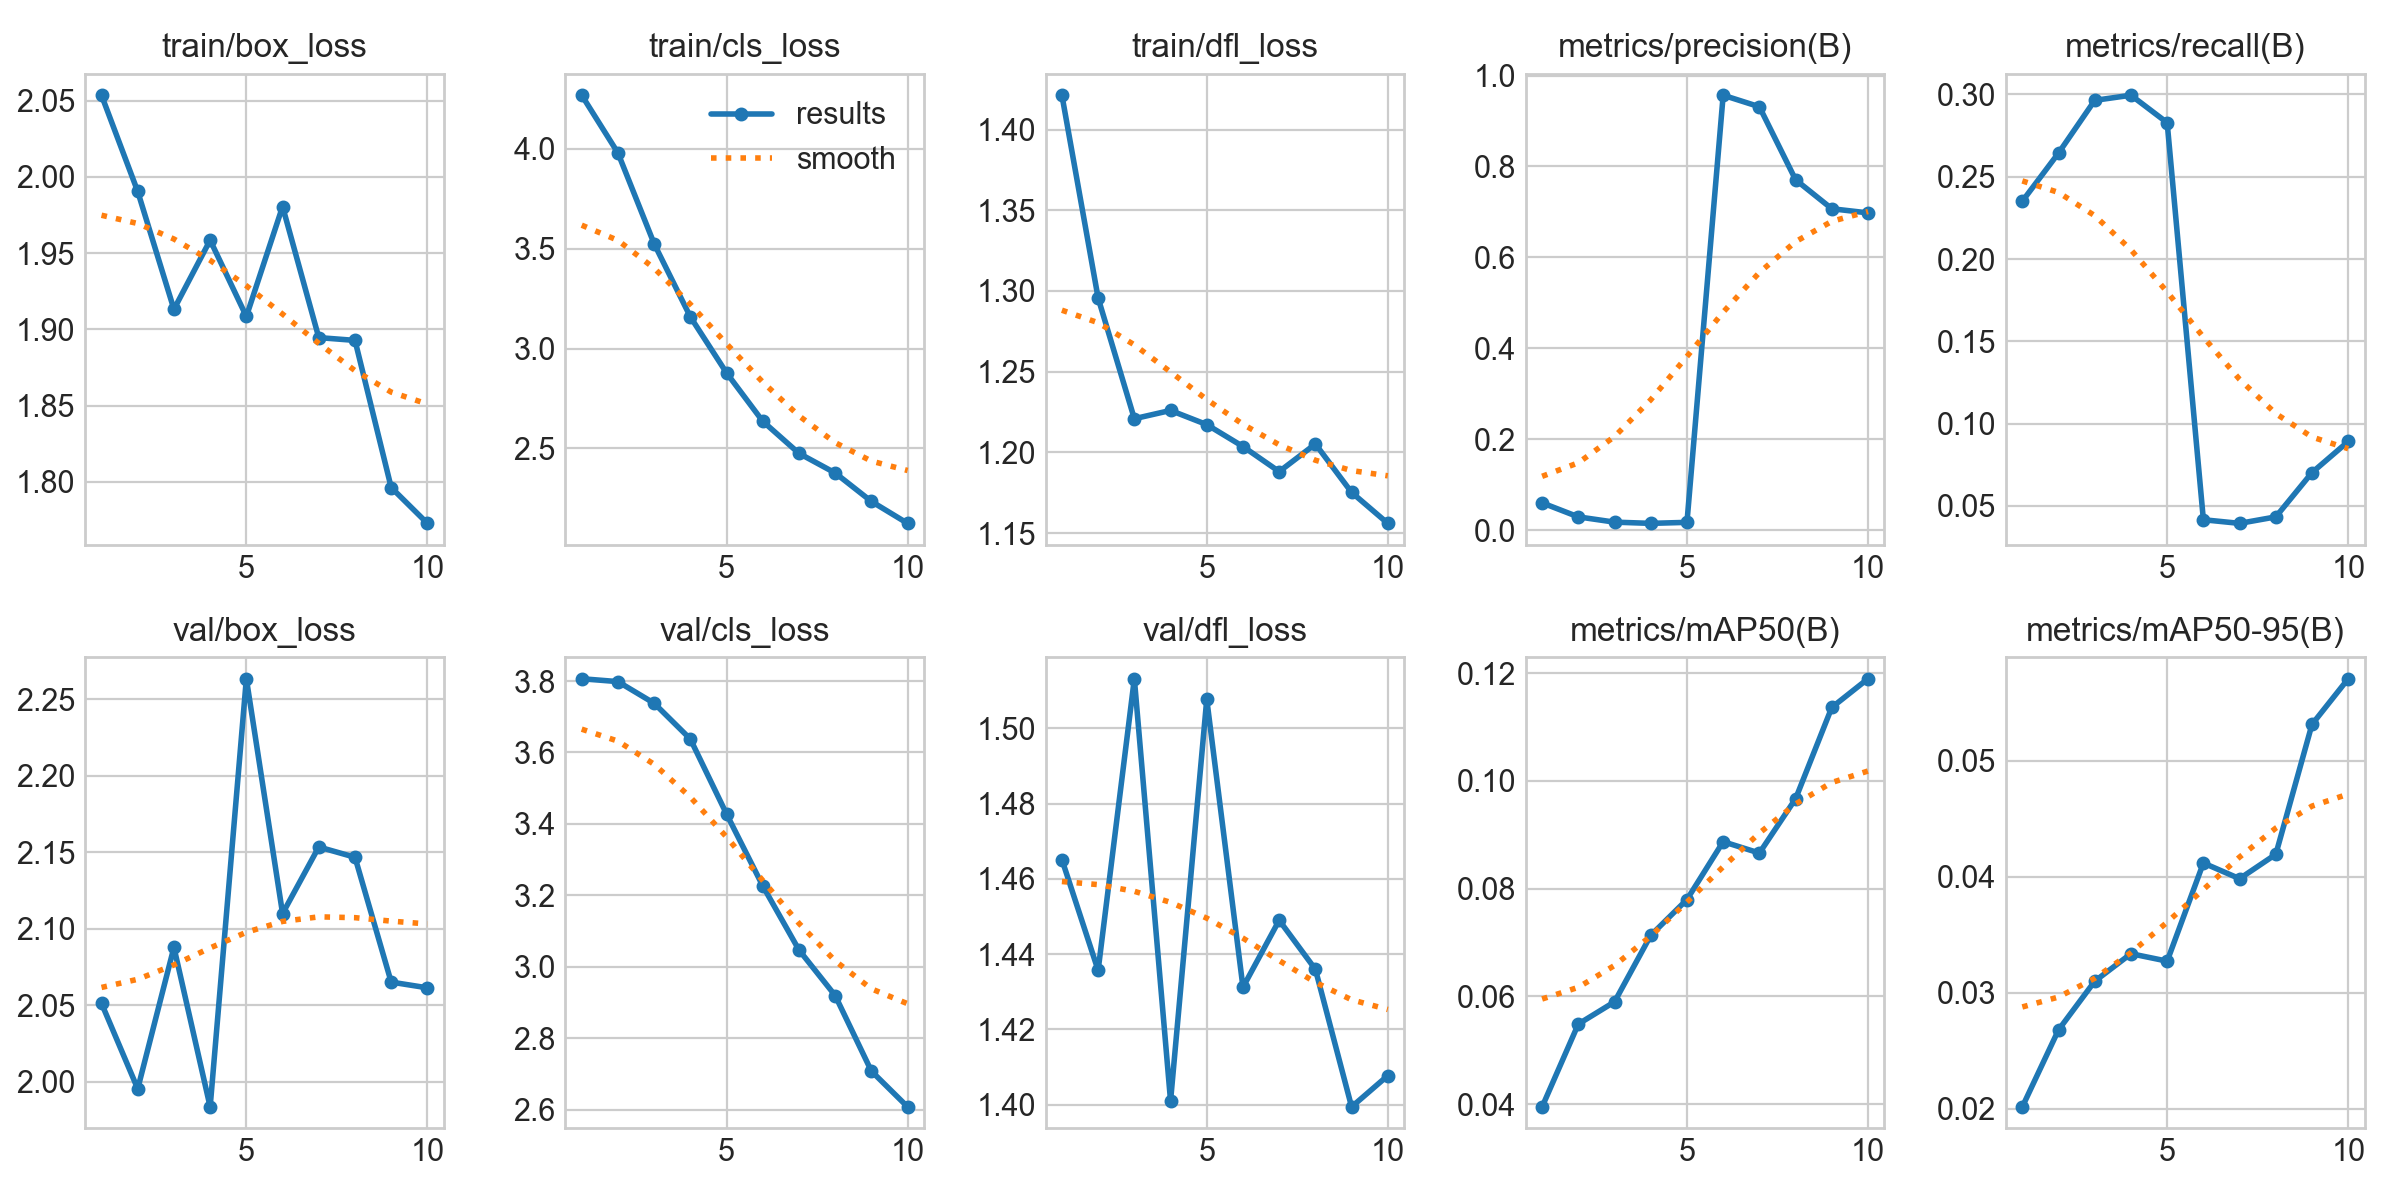
\includegraphics[width=\columnwidth]{figures/fig04_boston_curves.png}
\caption{YOLOv11n $C_1$ Boston fine-tune training curves.}
\label{fig:curves}
\end{figure}

\begin{figure}[htbp]
\centering
\begin{subfigure}[b]{0.82\columnwidth}
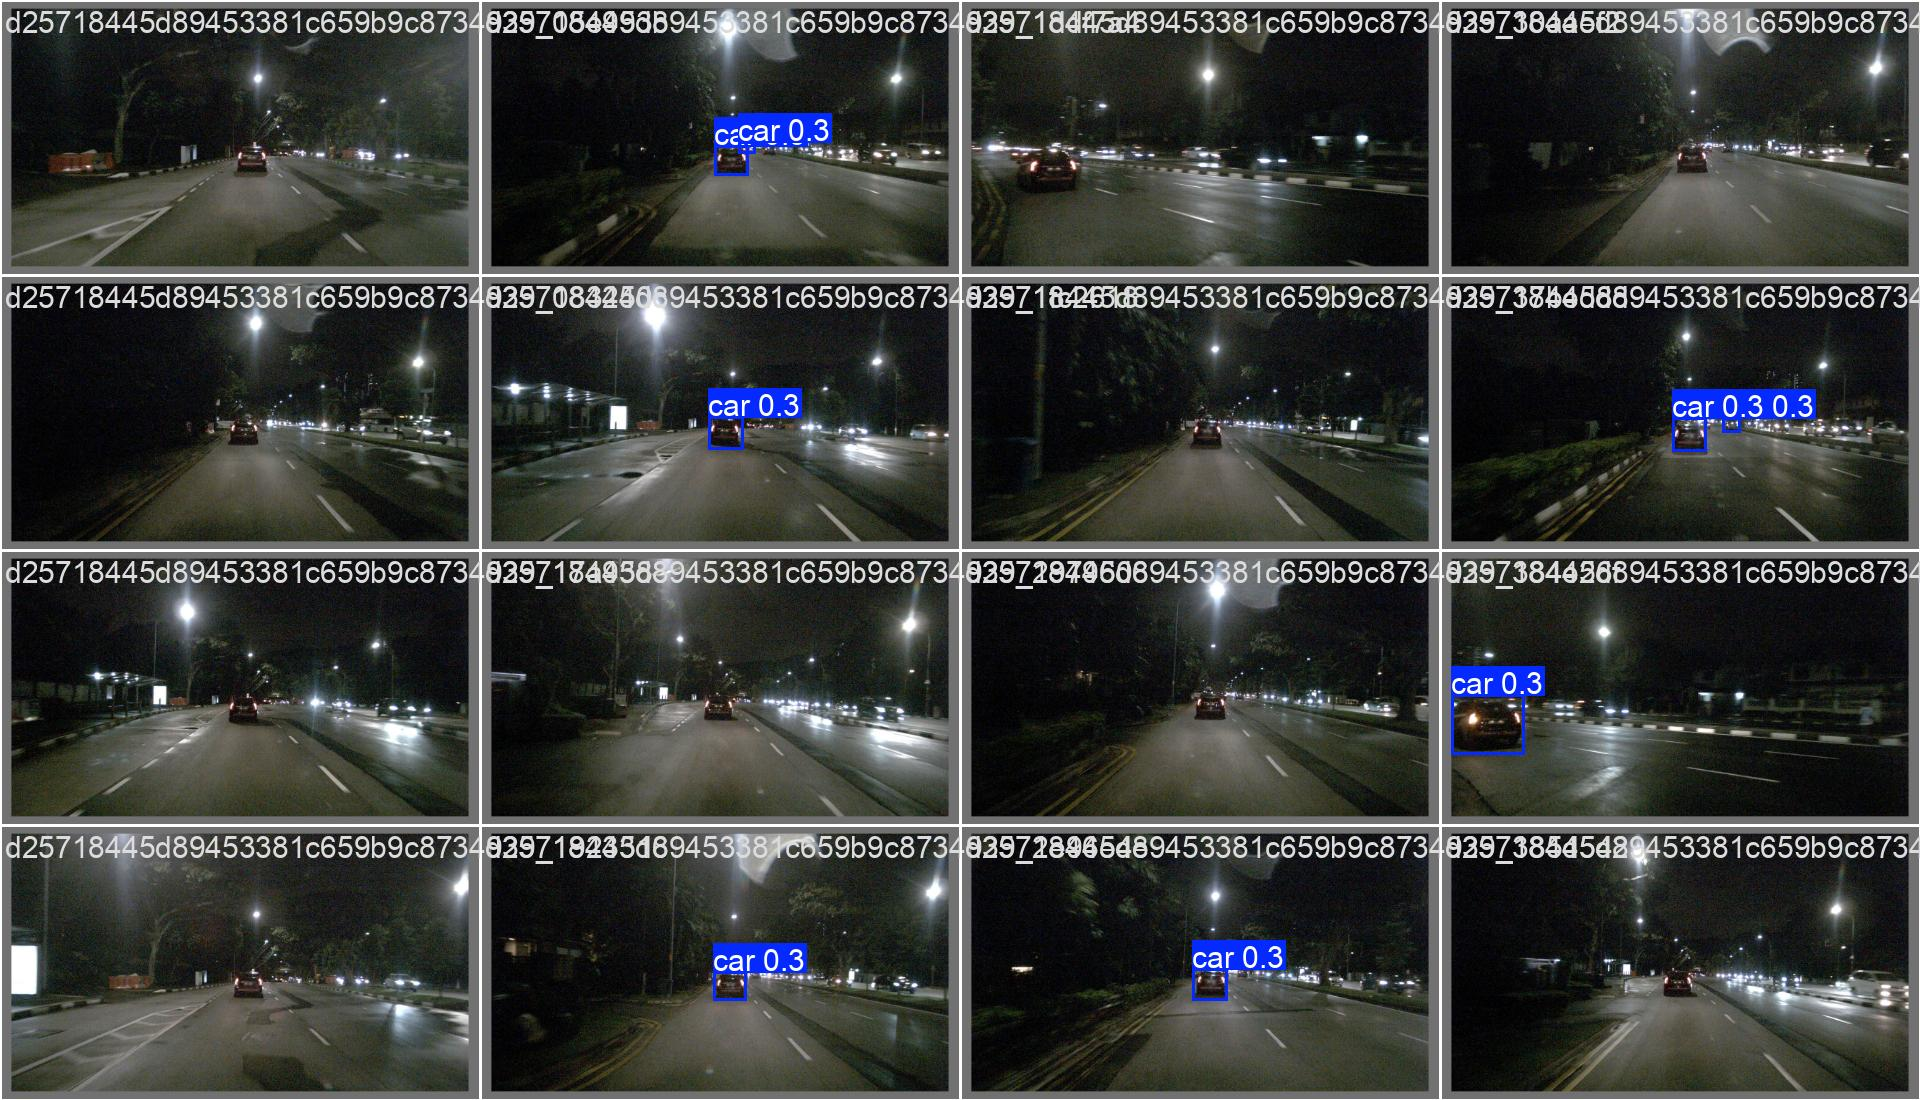
\includegraphics[width=\textwidth]{figures/fig05_singapore_val_pred.jpg}
\caption{Detections (predicted).}
\label{fig:qual-a}
\end{subfigure}

\vspace{1ex}

\begin{subfigure}[b]{0.82\columnwidth}
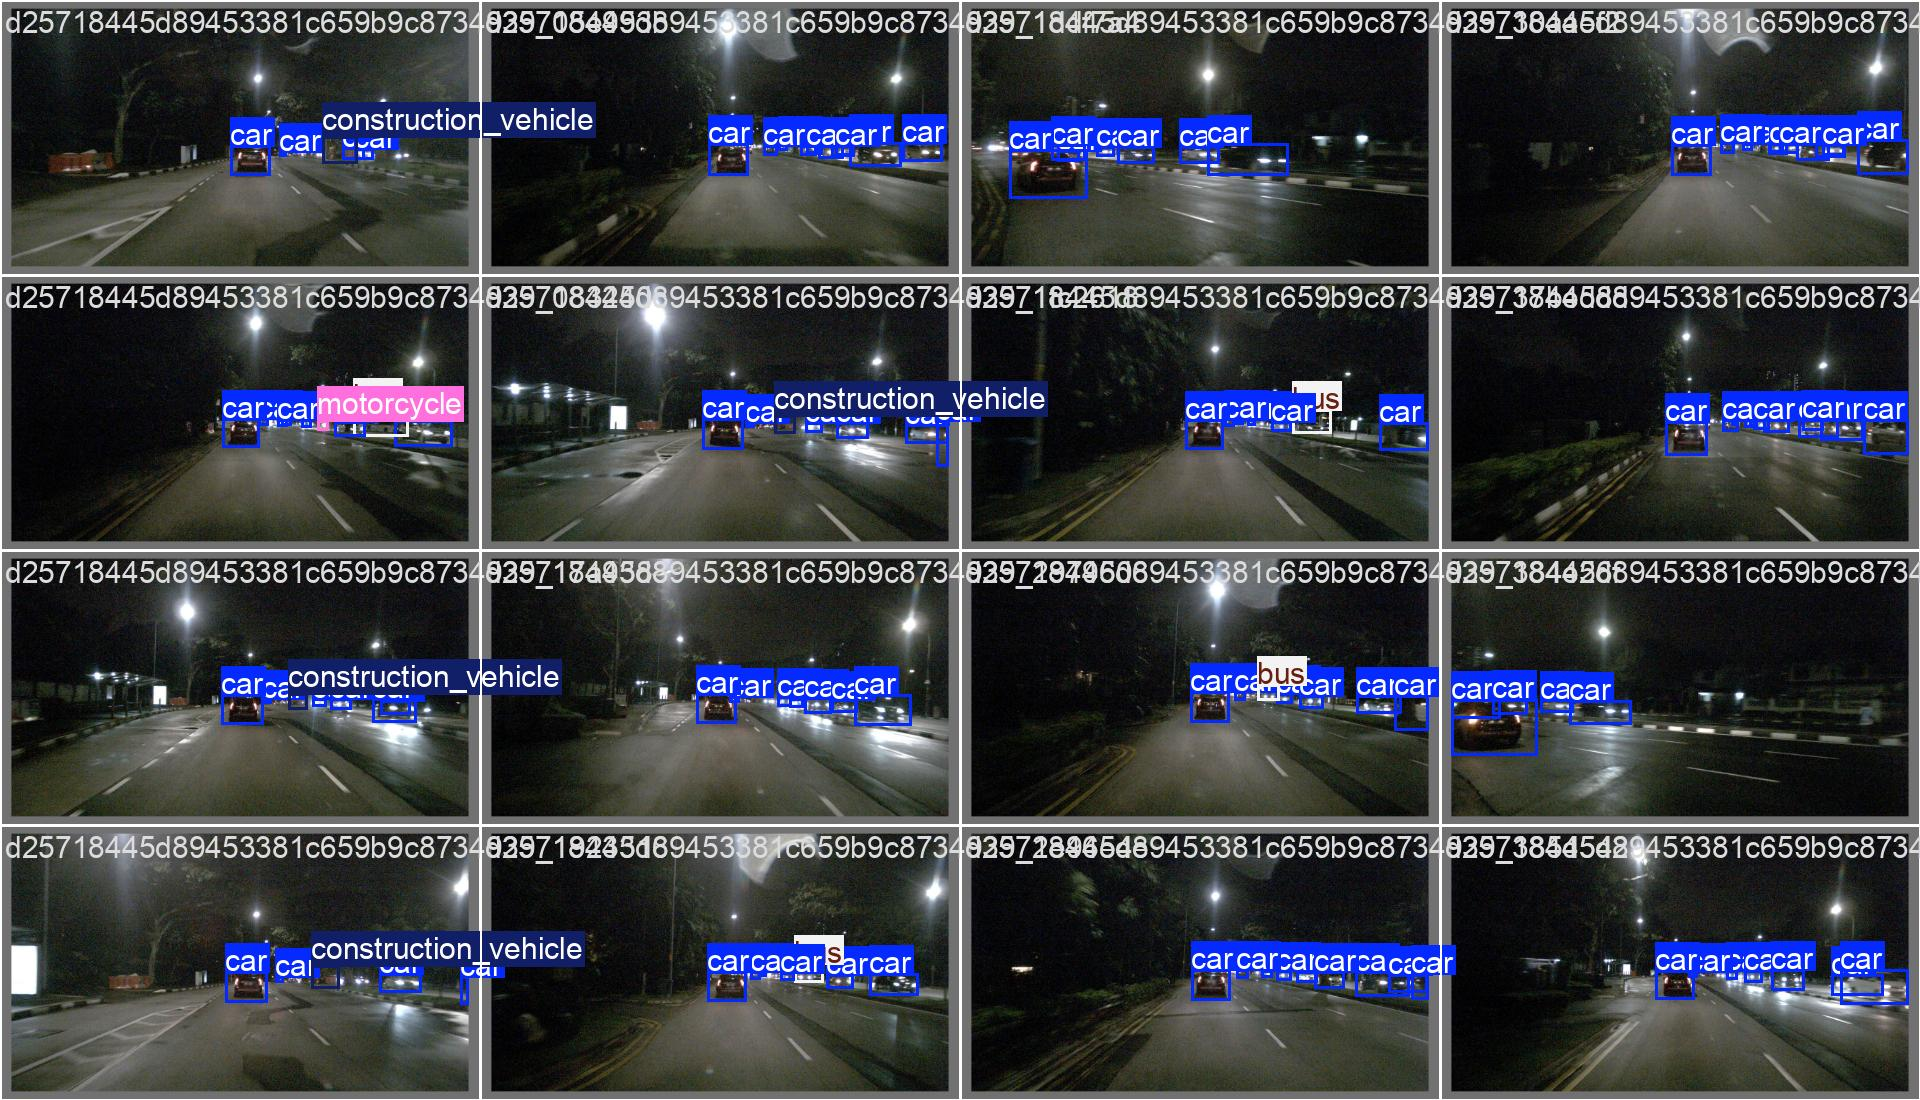
\includegraphics[width=\textwidth]{figures/fig05_singapore_val_labels.jpg}
\caption{Ground-truth labels.}
\label{fig:qual-b}
\end{subfigure}
\caption{Qualitative $C_1$ output on a Singapore validation batch.}
\label{fig:qual}
\end{figure}

% ============================================================================
\section{Discussion}
\label{sec:discussion}
% ============================================================================

\subsection{Mechanism of the Non-Monotone Cascade}
Under the Boston-trained C1, the planner's inputs were substantially displaced
($\Gamma_2 = 13.10$~m) in a regime whose errors the proposal-and-score rules
absorbed: missed or grossly misplaced agents leave the proximity penalty
inactive, so the planner follows its kinematic prior, which on these scenes
approximated the human trajectory. The fine-tuned C1 relocated detections near
their true positions and re-activated the penalty with correctly anchored but
coarse (zero-velocity) forecasts, causing the planner to react to obstacles it
had previously ignored. Downstream components can thus absorb upstream error,
and, symmetrically, upstream improvement can expose masked downstream
sensitivity, so a retrained component cannot be admitted on its own interface
alone.

\looseness=-1
This mechanism suggests the C3 regression may be a metric artifact rather than
a loss of driving quality. Collision rate was zero before and after
(Table~\ref{tab:results}), and the worse L2 arises because the improved
detector made the planner react to real agents instead of following a kinematic
prior that happened to track the recorded human path. This is the
ego-forecasting shortcut of nuScenes open-loop L2, under which
perception-agnostic prediction
is competitive~\cite{zhai2023rethinking} and open-loop error is weakly tied to
closed-loop quality~\cite{codevilla2018offline}. The update may thus be a
\emph{safer} planner that scores worse on a metric rewarding ignored
perception. This directly affects CARA (Section~\ref{sec:cara}): since its
admission rule keys on the terminal open-loop metric, it could reject a
genuinely improved update, so a closed-loop or NAVSIM-style
metric~\cite{dauner2024navsim} is the appropriate safeguard. Until then the
$+4.45\%$ should be read as reduced trajectory agreement, not an established
safety regression.

\subsection{Implications for MLS Maintenance Models}
The isolation check (F2) validates the per-component state factorization that
stochastic maintenance models assume. The injected cascades $\Delta_2 =
-11.24$~m and $\Delta_3 = +0.28$~m have opposite signs, demonstrating that a
single scalar ``retraining quality'' parameter is insufficient: one event can
act simultaneously as a repair for C2 and a fault injection for C3. Models of
imperfect retraining~\cite{wang2025issre} can represent this through
state-dependent transitions, which the coupling factor of
Section~\ref{sec:cara} is intended to calibrate once measured over updates with
an unambiguous $\delta_i$.

\subsection{Threats to Validity}
\label{sec:threats}
\textbf{Statistical power.} The validation set contains 3 scenes, one of which
dominates the C3 regression. The isolation rows establish that the $+4.45\%$
figure is a genuine measurement rather than apparatus noise, but its
generalization is not established; multi-seed replication and larger splits are
the direct remedy.

\textbf{Construct validity of open-loop L2.} As discussed in
Section~\ref{sec:discussion}, open-loop L2 rewards trajectory agreement over
safety, so the C3 result must be read differentially and confirmed with a
closed-loop or NAVSIM-style metric~\cite{dauner2024navsim} before any safety
claim.

\textbf{Component realism.} C2 is parameter-free and C1 is camera-based rather
than LiDAR~\cite{yin2021center}, and the IDM planner omits PDM-Closed's learned
scorer~\cite{dauner2023parting}; magnitudes will differ with richer components,
though the existence results (F2--F5) are architecture-independent.

\textbf{Small-data fine-tuning.} The mAP drop in F5 arises from a 119-image
fine-tune; a class-balanced fine-tune could flip the sign of $\delta_1$, which
would reinforce F5 (the decoupling claim) and, moreover, yield the unambiguous
$\delta_1$ that a clean $\rho$ requires.

% ============================================================================
\section{Proposed Method: Cascade-Aware Retraining Assessment}
\label{sec:cara}
% ============================================================================
The findings expose a concrete hazard: a retrained component that regresses on
its own metric may nonetheless improve its neighbor while degrading the system
(F4, F5), so neither component-level validation nor first-interface validation
is a sufficient admission criterion. We therefore generalize the measurement
method of this paper into an admission protocol for component updates in
modular MLS, termed Cascade-Aware Retraining Assessment (CARA), which formalizes
the procedure carried out manually in our experiment. Fig.~\ref{fig:cara}
summarizes the decision; the protocol is stated below.

\begin{figure}[htbp]
\centering
\resizebox{\columnwidth}{!}{%
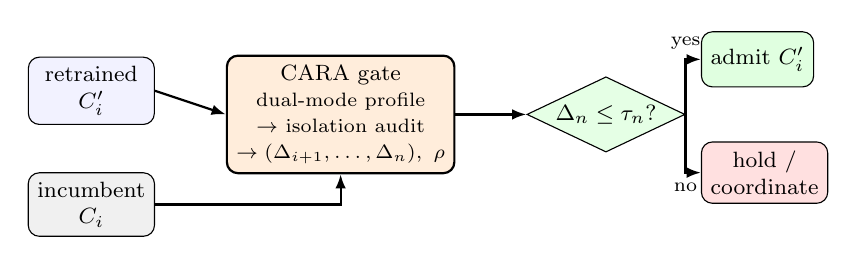
\begin{tikzpicture}[
    font=\footnotesize,
    node distance=5mm,
    box/.style={draw, rounded corners, minimum height=7mm, minimum width=16mm,
                align=center, fill=blue!5},
    old/.style={draw, rounded corners, minimum height=7mm, minimum width=16mm,
                align=center, fill=black!6},
    gate/.style={draw, rounded corners, minimum height=10mm, minimum width=26mm,
                 align=center, fill=orange!14, thick},
    dec/.style={draw, diamond, aspect=2.1, align=center, fill=green!10, inner sep=1pt},
    pass/.style={draw, rounded corners, minimum height=7mm, align=center, fill=green!12},
    stop/.style={draw, rounded corners, minimum height=7mm, align=center, fill=red!12},
    arr/.style={-{Latex[length=1.8mm]}, thick}
]
\node[box] (new) {retrained\\$C_i'$};
\node[old, below=6mm of new] (old) {incumbent\\$C_i$};
\node[gate, right=9mm of new, yshift=-3mm] (gate)
     {CARA gate\\\scriptsize dual-mode profile\\\scriptsize $\to$ isolation audit\\\scriptsize $\to (\Delta_{i+1},\dots,\Delta_n),\ \rho$};
\node[dec, right=9mm of gate] (dec) {$\Delta_n \le \tau_n$?};
\node[pass, above right=1mm and 7mm of dec] (pass) {admit $C_i'$};
\node[stop, below right=1mm and 7mm of dec] (stop) {hold /\\coordinate};
\draw[arr] (new.east) -- (gate.west);
\draw[arr] (old.east) -| ($(gate.south)$);
\draw[arr] (gate) -- (dec);
\draw[arr] (dec.east) |- (pass.west) node[midway,above,font=\scriptsize]{yes};
\draw[arr] (dec.east) |- (stop.west) node[midway,below,font=\scriptsize]{no};
\end{tikzpicture}%
}
\caption{The CARA admission gate for a retrained component.}
\label{fig:cara}
\end{figure}

\subsection{Protocol}
Given a pipeline $C_1 \to \dots \to C_n$, a frozen audit set $A$, and a
candidate update $R$ to component $C_i$, CARA proceeds as follows
(Algorithm~\ref{alg:cara}). With the incumbent $C_i$ it records the dual-mode
profile $P_{\text{before}} = \{ M_k^{\text{iso}}, M_k^{\text{pipe}} : k=i..n \}$
on $A$, then swaps in the retrained $C_i'$ and records $P_{\text{after}}$ on the
identical audit set with fixed randomness. It requires
$M_k^{\text{iso}}(\text{before}) = M_k^{\text{iso}}(\text{after})$ for every
frozen $C_k$; any violation signals leakage or nondeterminism and invalidates
the assessment (in our experiment this audit passed bit-exactly, F2). It then
computes the injected cascade $\Delta_k$~\eqref{eq:inj} at every downstream
component and reports the full vector $(\Delta_{i+1}, \dots, \Delta_n)$, since
adjacent deltas can carry opposite signs, together with the cascade coupling
factor of Section~\ref{sec:diag}, generalized to an update on any component,
\begin{equation}
\rho_{i \to n} = \frac{\Delta_n}{\delta_i}.
\label{eq:rho}
\end{equation}
A negative $\rho$ with an improving $\delta_i$ is the entangled-enhancement
regime. We stress that $\rho$ is well-defined only when $\delta_i$ is
unambiguous; in our single experiment $\delta_1 < 0$, so $\rho_{1\to 3}$ is of
ambiguous sign and is not cleanly measurable, and a meaningful value requires an
update whose component metric moves definitely, such as the class-balanced C1
fine-tune of Section~\ref{sec:conclusion}. Finally, $C_i'$ is admitted only if
$\Delta_n \le \tau_n$ and safety-critical auxiliaries such as collision rate do
not regress; if $\Delta_n > \tau_n$ while intermediate interfaces improve, as in
the observed pattern, the update is held or routed to coordinated retraining of
the downstream consumers, converting a single-component update into a
coordinated multi-component transition.

\begin{algorithm}[htbp]
\SetAlgoLined
\DontPrintSemicolon
\KwIn{pipeline $C_1\!\to\!\dots\!\to\!C_n$; audit set $A$; candidate update
$R$ on $C_i$; tolerance $\tau_n$}
\KwOut{admit / hold decision, cascade vector, coupling factor $\rho$}
$P_{\text{before}} \leftarrow \textsc{DualModeProfile}(C_i, A)$\;
$C_i' \leftarrow R(C_i)$;\quad
$P_{\text{after}} \leftarrow \textsc{DualModeProfile}(C_i', A)$\;
\ForEach{frozen $C_k$, $k>i$}{
  \If{$M_k^{\text{iso}}(\text{after}) \ne M_k^{\text{iso}}(\text{before})$}{
    \Return \textbf{invalid} \tcp*{isolation violated (contamination)}
  }
}
$\Delta_k \leftarrow M_k^{\text{pipe}}(\text{after})-M_k^{\text{pipe}}(\text{before})$
for $k=i{+}1..n$\;
$\rho \leftarrow \Delta_n / \delta_i$\;
\eIf{$\Delta_n \le \tau_n$ \textbf{and} collision rate not worse}{
  \Return \textbf{admit} $C_i'$\;
}{
  \Return \textbf{hold} / coordinate downstream retraining\;
}
\caption{Cascade-Aware Retraining Assessment (CARA)}
\label{alg:cara}
\end{algorithm}

\subsection{Mitigation of the Observed Failure Modes}
\looseness=-1
Admission never rests on $\delta_i$ (addressing F5) and reports the full delta
vector, so an improvement at C2 cannot mask a regression at C3 (addressing F4).
The isolation audit in Step 3 makes silent contamination detectable by exact
equality testing, a check available only because the architecture is modular
(F1), and CARA's marginal cost is inference on a fixed audit set with no
training. In an E2E monolith Steps 1--5 are undefined, since there are no frozen
components, isolated modes, or interfaces at which $\Delta_k$ could be measured,
so the protocol is constructible only in the modular setting.

\subsection{Positioning}
CARA is largely the experimental procedure of this paper cast as an explicit
gate; its contribution is not a new algorithm but the gate statistic, a
per-interface cascade vector with a terminal admission threshold and an
isolation audit, in place of input-data drift scores~\cite{breck2019data}
alone. It is complementary to regression-constrained
retraining~\cite{yan2021pctraining,shen2020bct}, which \emph{reduces} the
cascade that CARA \emph{measures}, and to uncertainty-propagating
interfaces~\cite{ivanovic2022propagating} that absorb the residual.

% ============================================================================
\section{Conclusion and Future Work}
\label{sec:conclusion}
% ============================================================================
We presented a controlled study of single-component retraining in a modular
perception--prediction--planning pipeline under a geographic domain shift.
Under dual-mode evaluation with a verified isolation control, retraining C1
improved C2 by 73.98\% in pipeline mode while C3 degraded by 4.45\% and C1's
aggregate metric moved opposite to its interface usefulness. These findings,
from the architectural necessity of modularity to aggregate-metric decoupling,
show that component-level validation is insufficient for safe MLS maintenance,
which the CARA protocol addresses at inference-only cost. The broader
contribution is methodological: cascade effects can be measured under exact
controls, but only in an architecture that exposes its interfaces.

Future work runs along four lines: statistical hardening with multi-seed
replication and larger splits; class-balanced fine-tuning of C1, which both
tests the entangled-enhancement signature and yields the unambiguous $\delta_1$
a clean $\rho$ requires; full coverage of the seven-subset retraining lattice
over $\{$C1, C2, C3$\}$, calibrating the base paper's stochastic maintenance
models~\cite{wang2024compsac,wang2025issre}; and moving C1 to LiDAR
detection~\cite{yin2021center} with NAVSIM-style
scoring~\cite{dauner2024navsim} for C3.

\bibliographystyle{IEEEtran}
\bibliography{references}
\end{document}
